%\documentclass[
  bibliography=totoc,     % Literatur im Inhaltsverzeichnis
  captions=tableheading,  % Tabellenüberschriften
  titlepage=firstiscover, % Titelseite ist Deckblatt
]{scrartcl}

% Paket float verbessern
\usepackage{scrhack}

% Warnung, falls nochmal kompiliert werden muss
\usepackage[aux]{rerunfilecheck}

% unverzichtbare Mathe-Befehle
\usepackage{amsmath}
% viele Mathe-Symbole
\usepackage{amssymb}
% Erweiterungen für amsmath
\usepackage{mathtools}

% Fonteinstellungen
\usepackage{fontspec}
% Latin Modern Fonts werden automatisch geladen
% Alternativ zum Beispiel:
%\setromanfont{Libertinus Serif}
%\setsansfont{Libertinus Sans}
%\setmonofont{Libertinus Mono}

% Wenn man andere Schriftarten gesetzt hat,
% sollte man das Seiten-Layout neu berechnen lassen
\recalctypearea{}

% deutsche Spracheinstellungen
\usepackage[ngerman]{babel}


\usepackage[
  math-style=ISO,    % ┐
  bold-style=ISO,    % │
  sans-style=italic, % │ ISO-Standard folgen
  nabla=upright,     % │
  partial=upright,   % │
  mathrm=sym,        % ┘
  warnings-off={           % ┐
    mathtools-colon,       % │ unnötige Warnungen ausschalten
    mathtools-overbracket, % │
  },                       % ┘
]{unicode-math}

% traditionelle Fonts für Mathematik
\setmathfont{Latin Modern Math}
% Alternativ zum Beispiel:
%\setmathfont{Libertinus Math}

\setmathfont{XITS Math}[range={scr, bfscr}]
\setmathfont{XITS Math}[range={cal, bfcal}, StylisticSet=1]

% Zahlen und Einheiten
\usepackage[
  locale=DE,                   % deutsche Einstellungen
  separate-uncertainty=true,   % immer Unsicherheit mit \pm
  per-mode=symbol-or-fraction, % / in inline math, fraction in display math
]{siunitx}

% chemische Formeln
\usepackage[
  version=4,
  math-greek=default, % ┐ mit unicode-math zusammenarbeiten
  text-greek=default, % ┘
]{mhchem}

% richtige Anführungszeichen
\usepackage[autostyle]{csquotes}

% schöne Brüche im Text
\usepackage{xfrac}

% Standardplatzierung für Floats einstellen
\usepackage{float}
\floatplacement{figure}{htbp}
\floatplacement{table}{htbp}

% Floats innerhalb einer Section halten
\usepackage[
  section, % Floats innerhalb der Section halten
  below,   % unterhalb der Section aber auf der selben Seite ist ok
]{placeins}

% Seite drehen für breite Tabellen: landscape Umgebung
\usepackage{pdflscape}

% Captions schöner machen.
\usepackage[
  labelfont=bf,        % Tabelle x: Abbildung y: ist jetzt fett
  font=small,          % Schrift etwas kleiner als Dokument
  width=0.9\textwidth, % maximale Breite einer Caption schmaler
]{caption}
% subfigure, subtable, subref
\usepackage{subcaption}

% Grafiken können eingebunden werden
\usepackage{graphicx}

% schöne Tabellen
\usepackage{tabularray}
\UseTblrLibrary{booktabs, siunitx}

% Verbesserungen am Schriftbild
\usepackage{microtype}

% Literaturverzeichnis
\usepackage[
  backend=biber,
]{biblatex}
% Quellendatenbank
\addbibresource{lit.bib}
\addbibresource{programme.bib}

% Hyperlinks im Dokument
\usepackage[
  german,
  unicode,        % Unicode in PDF-Attributen erlauben
  pdfusetitle,    % Titel, Autoren und Datum als PDF-Attribute
  pdfcreator={},  % ┐ PDF-Attribute säubern
  pdfproducer={}, % ┘
]{hyperref}
% erweiterte Bookmarks im PDF
\usepackage{bookmark}

% Trennung von Wörtern mit Strichen
\usepackage[shortcuts]{extdash}

\author{%
  Vincent Wirsdörfer\\%
  \href{mailto:vincent.wirsdoerfer@udo.edu}{authorA@udo.edu}%
  \and%
  Joris Daus\\%
  \href{mailto:joris.daus@udo.edu}{authorB@udo.edu}%
}
\publishers{TU Dortmund – Fakultät Physik}


%\begin{document}
\section{Diskussion}
\label{sec:Diskussion}

Wie bereits in der Einleitung des Protokolls erwähnt, besteht das Ziel darin, das magnetische Moment des Permanentmagneten
auf verschiedene experimentelle Wege zu bestimmen. Um die bestimmten Werte des magnetischen Dipolmomentes miteinander 
vergleichen zu können, werden Diese im Folgenden aufgelistet.

\begin{align*}
    \mu_\text{Gravitation} &= \left(0.480 \pm 0.031\right)\,\unit{\ampere\meter\squared} \\
    \mu_\text{Schwingung} &= \left(0.299 \pm 0.09\right)\,\unit{\ampere\meter\squared} \\
    \mu_\text{Präzession} &= \left(0.42 \pm 0.04\right)\,\unit{\ampere\meter\squared} \\
\end{align*}

\noindent Die relativen Abweichungen der einzelnen Werte berechnen sich über die Formel 

\begin{equation*}
    \increment\mu_{1,2} = \frac{\mu_1 - \mu_2}{\mu_2}.
\end{equation*}

\noindent Das bedeutet konkret für die jeweiligen Abweichungen:

\begin{align*}
    \increment\mu_\text{Grav,Schwing} &\approx 60.54\,\unit{\percent} \\
    \increment\mu_\text{Grav,Präz} &\approx 14.29\,\unit{\percent} \\
    \increment\mu_\text{Schwing,Präz} &\approx 28.81\,\unit{\percent} \\
\end{align*}

\noindent Die genauen Ursachen für die relativen Abweichungen der Werte lassen sich nicht erklären, da beispielsweise 
potentiellen Fehlerquellen der Gravitationsmethode dazu führen könnten, dass die relative Abweichung der Werte aus der 
Gravitation näher an dem Wert der Präzessionsmethode liegen. \\
Dessen ungeachtet können allgemeine Fehlerquellen benannt werden, welche zu einer Abweichung vom Theoriewert führen. Dieser 
Theoriewert ist jedoch nicht gegeben, weswegen kein direkter Vergleich stattfinden kann.\\\\
Eine mögliche Fehlerquelle der Gravitationsmethode besteht in der Unbeständigkeit des Luftkissens. Sehr häufig musste 
die Kugel durch leichte Berührungen vom Kontakt mit der Messing-Halbschale getrennt werden, sodass die Kugel erneut 
auf dem Luftkissen schwebt. Dadurch konnte nur schwierig festgestellt werden, ab welcher Stromstärke, beziehungsweise ab 
welcher Magnetfeldstärke ein Gleichgewicht der Drehmomente vorliegt. Zusätzlich ist das Erreichen des Gleichgewichts 
ein \enquote{feinfühliger} Prozess, was nicht in der groben Skalierung der Stromstärke berücksichtigt wird. Im Zusammenhang 
mit Parallaxenfehlern korreliert die gemessene Stromstärke somit nicht komplett mit dem Gleichgewicht des Systems.\\
Auch wenn der potentiell größte Fehler der Schwingungsmethode durch die Messung von zehn Zeitperioden weggemittelt wird,
fließen auch hier systematische Fehler in das Endergebnis ein. Zum Einen kann nicht zu $100\,\unit{\percent}$ 
gewährleistet werden, dass die Auslenkung des Stabes hinreichend klein ist. Dies ist jedoch essenziell für die 
Berechnungsmethode, da nur in Kleinwinkelnäherung ein harmonischer Oszillator beschrieben wird. Zum Anderen wird die Zeit 
der Periodendauern per Hand gemessen, was durchaus zu Ungenauigkeiten und Unterschieden zwischen einzelnen Messungen 
führen kann. \\
Die wahrscheinlich komplexeste Methode ist die Bestimmung des Dipolmomentes mittels der Präzession der Billardkugel.
Dementsprechend lässt sich hierbei ein breites Spektrum an Fehlerquellen nennen. Wie im vorherigen Kapitel \ref{sec:Durchfuehrung}
bereits beschrieben, muss die Kreisfrequenz der Kugel an die des Stroboskops angepasst werden. Aufgrund von Luftreibung,
leichten Nutationsphänomenen und verschiedenen Lichteinfallswinkeln ist dies jedoch nur schwer umsetzbar. Auch wenn der weiße
Punkt auf dem Stiel für einen Augenblick stationär erscheint, so ist es schwierig, eine Frequenz zu treffen, welche über 
die gesamte Präzessionsdauer parallel zur Frequenz des Stroboskops ist. Außerdem führt die Frequenzverringerung der Kugel 
durch Luftreibung dazu, dass nach Erreichen des Stroboskopfrequenz, schnellstmöglich eine bestimmte Stromstärke eingestellt werden 
muss, was potentielle Parallaxenfehler bestärkt. \\\\
Somit weisen alle Methoden mögliche Fehlerquellen auf, welche die Messung der Dipolmomente beeinflussen.

\section{Anhang}

\begin{figure}[H]
    \centering
    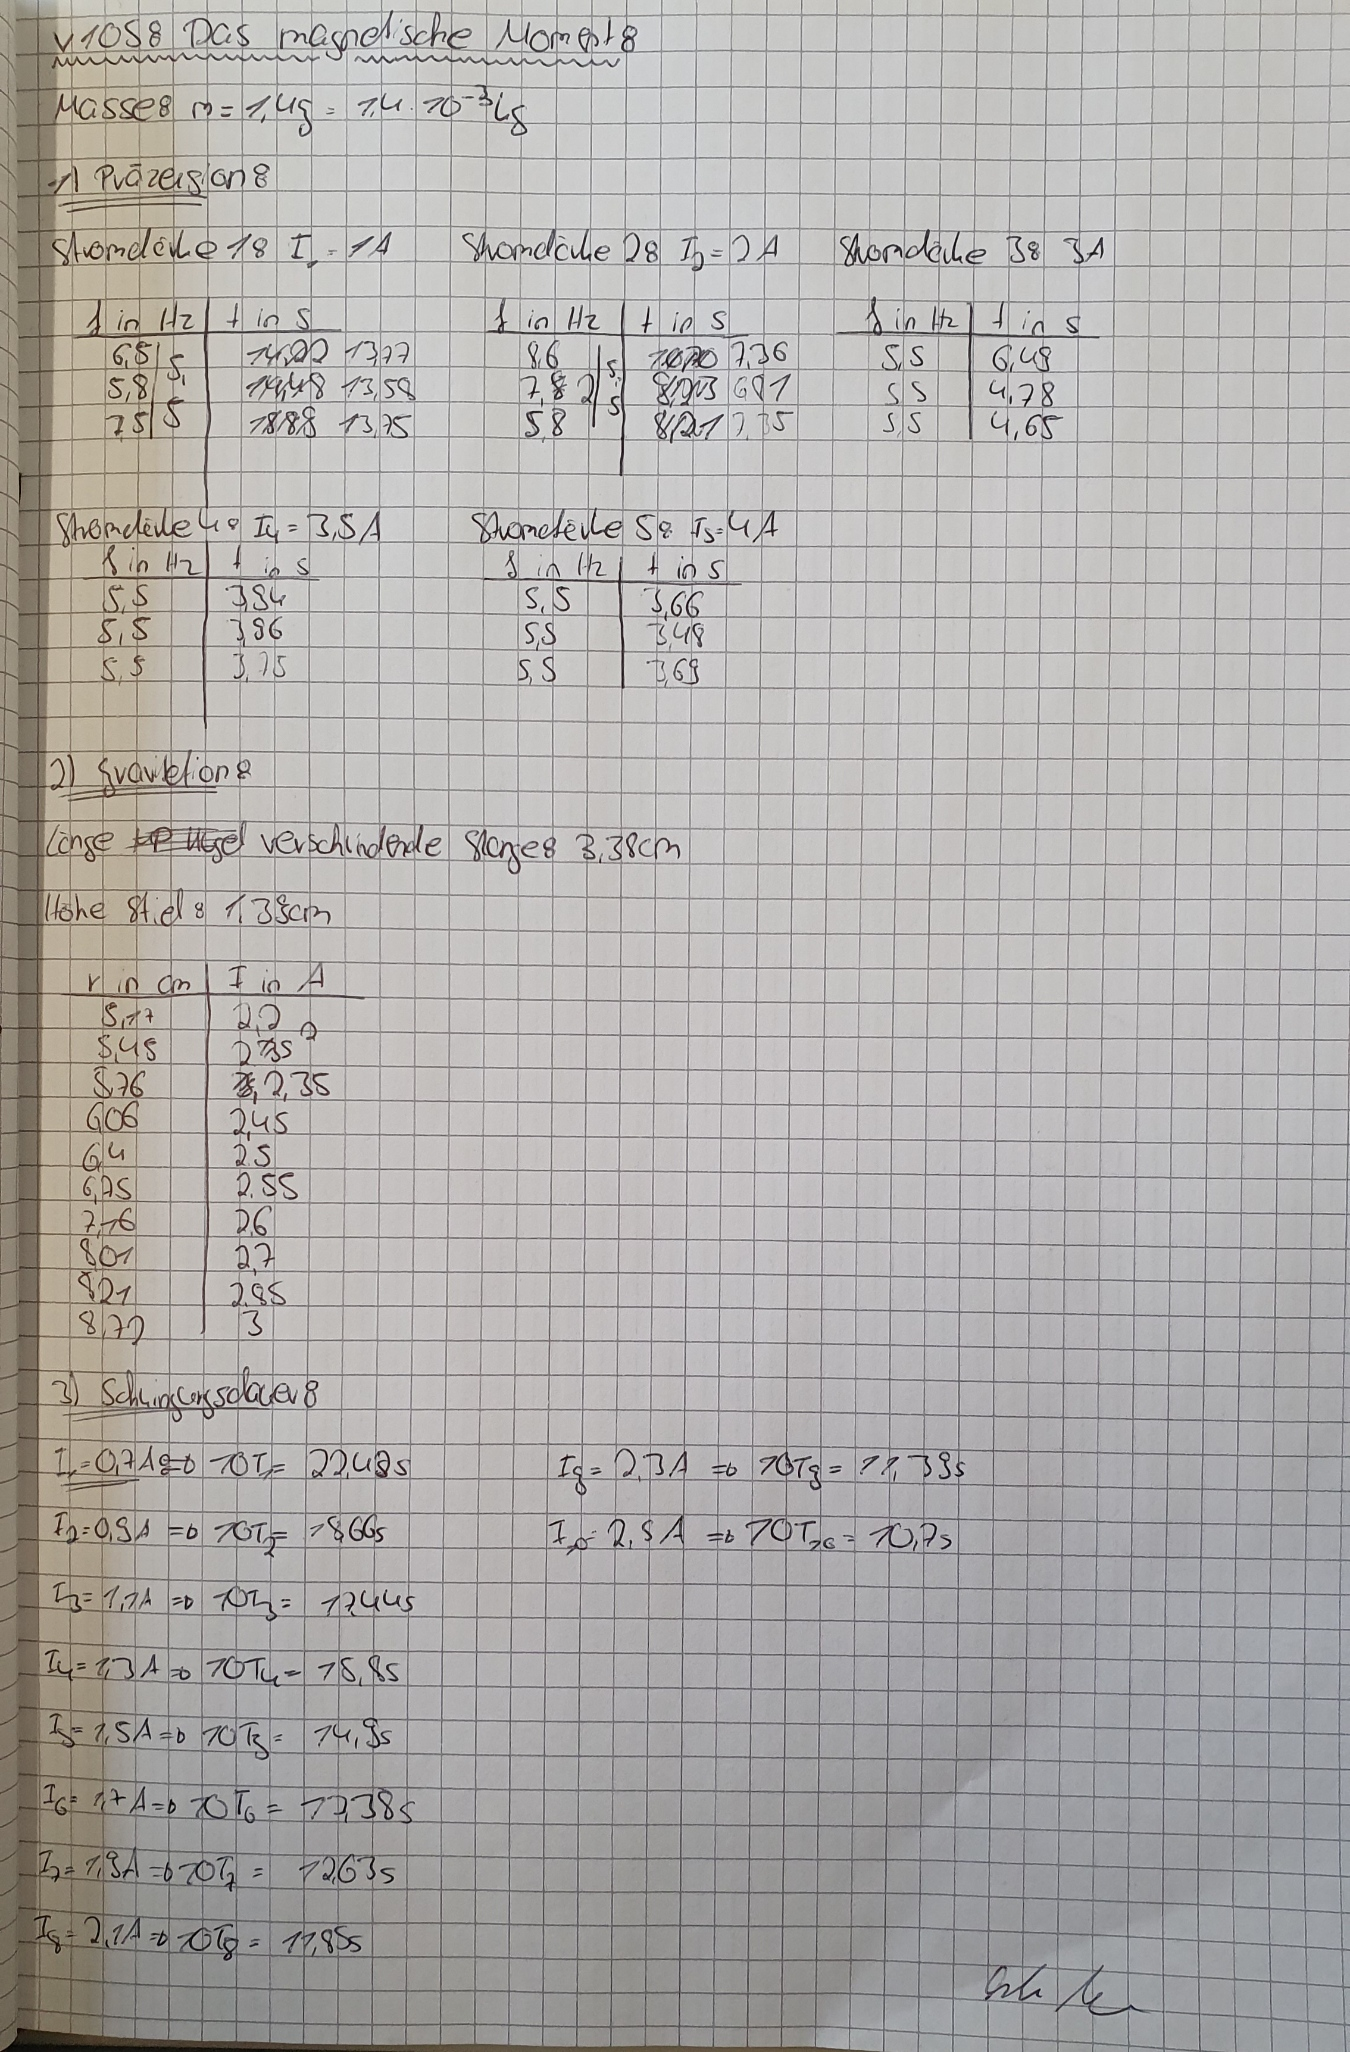
\includegraphics[width=\textwidth]{Daten.jpg}
    \caption{Originalmesswerte des Versuchs.}
\end{figure}

%\end{document}
